\documentclass{ansarticle-preprint}
%\usepackage{ucs}
\usepackage[utf8]{inputenc}
\usepackage{amsmath}
%\usepackage{cite}
\usepackage{anslistings}
\usepackage{multicol}
\usepackage{pdfsync}

\usepackage{pgfplots}
\usepackage{pgfplotstable}

\usepackage{fontenc}
\usepackage{graphicx}
\usepackage{xspace}

\usepackage{siunitx}

\usepackage{floatflt}

\usepackage{multirow}

%\renewcommand{\baselinestretch}{2.0}

\graphicspath{{svg/}}

\usepackage[normalem]{ulem}

\usepackage{caption}
\usepackage{subcaption}

\usepackage{todonotes}

\pgfplotsset{compat=1.9}
\definecolor{gnuplot@lightblue}{RGB}{87,181,232}
\definecolor{gnuplot@green}{RGB}{0,158,115}
\definecolor{gnuplot@purple}{RGB}{148,0,212}

\newcommand{\specialword}[1]{\texttt{#1}}
\newcommand{\dealii}{{\specialword{deal.II}}\xspace}
\newcommand{\pfrst}{{\specialword{p4est}}\xspace}
\newcommand{\trilinos}{{\specialword{Trilinos}}\xspace}
\newcommand{\aspect}{\specialword{Aspect}\xspace}
\newcommand{\petsc}{\specialword{PETSc}\xspace}
\newcommand{\cmake}{{\specialword{CMake}}\xspace}
\newcommand{\candi}{{\specialword{candi}}\xspace}



\usetikzlibrary{shapes.misc}
\tikzset{cross/.style={cross out, draw=black, minimum size=2*(#1-\pgflinewidth), inner sep=0pt, outer sep=0pt},
%default radius will be 1pt.
cross/.default={2pt}}

%
% Author list -- please add yourself in both places below (in
%                alphabetical order) if you think that your
%                contributions to the last release warrant this
%

\hypersetup{
  pdfauthor={
    Daniel Arndt,
    Wolfgang Bangerth,
    Marco Feder,
    Marc Fehling,
    Timo Heister,
    Luca Heltai,
    Martin Kronbichler,
    Matthias Maier,
    Peter Munch,
    Jean-Paul Pelteret,
    Simon Sticko,
    Bruno Turcksin,
    David Wells
  },
  pdftitle={The deal.II Library, Version 9.4, 2022},
}

\title{The \dealii{} Library, Version 9.4}

 \author[1*]{Daniel Arndt}
 \affil[1]{Scalable Algorithms and Coupled Physics Group,
   Computational Sciences and Engineering Division,
   Oak Ridge National Laboratory, 1 Bethel Valley Rd.,
   TN 37831, USA.
   \texttt{arndtd/turcksinbr@ornl.gov}}

 \author[2,3]{Wolfgang~Bangerth}
 \affil[2]{Department of Mathematics, Colorado State University, Fort
   Collins, CO 80523-1874, USA.
   \texttt{bangerth/marc.fehling@colostate.edu}}
 \affil[3]{Department of Geosciences, Colorado State University, Fort
   Collins, CO 80523, USA.}

   \author[4]{Marco~Feder}
\affil[4]{SISSA,
   International School for Advanced Studies,
   Via Bonomea 265,
   34136, Trieste, Italy.
   {\texttt{ \{marco.feder,luca.heltai\}@sissa.it}}}

\author[2]{Marc~Fehling}

\author[5]{Timo~Heister}
 \affil[5]{School of Mathematical and Statistical Sciences,
   Clemson University,
   Clemson, SC, 29634, USA
   {\texttt{heister@clemson.edu}}}

\author[4]{Luca~Heltai}

 \author[6,7]{Martin~Kronbichler}
 \affil[6]{Department of Information Technology,
   Uppsala University,
   Box 337, 751\,05 Uppsala, Sweden.
   {\texttt{martin.kronbichler/simon.sticko@it.uu.se}}}
 \affil[7]{Institute of Mathematics,
   University of Augsburg,
   Universit\"atsstr.~12a, 86159 Augsburg, Germany.
   {\texttt{martin.kronbichler@uni-a.de}}}

\author[8]{Matthias~Maier}
\affil[8]{Department of Mathematics,
  Texas A\&M University,
  3368 TAMU,
  College Station, TX 77845, USA.
  {\texttt{maier@math.tamu.edu}}}

\author[7,9]{Peter Munch}
 \affil[9]{Institute of Material Systems Modeling,
 Helmholtz-Zentrum Hereon,
 Max-Planck-Str. 1, 21502 Geesthacht, Germany.
   {\texttt{peter.muench@hereon.de}}}


\author[10]{Jean-Paul~Pelteret}
\affil[10]{Independent researcher.
{\texttt{jppelteret@gmail.com}}}

\author[6,11]{Simon~Sticko}
\affil[11]{Department of Mathematics and Mathematical Statistics,
   Umeå University,
   SE-90187 Umeå, Sweden}

\author[1*]{Bruno~Turcksin}

\author[12]{David Wells}
\affil[12]{Department of Mathematics, University of North Carolina,
  Chapel Hill, NC 27516, USA.
  {\texttt{drwells@email.unc.edu}}}

\renewcommand{\labelitemi}{--}


\begin{document}
\maketitle

\footnotetext{%
  $^\ast$ This manuscript has been authored by UT-Battelle, LLC under Contract No.
  DE-AC05-00OR22725 with the U.S. Department of Energy.
  %The United States
  %Government retains and the publisher, by accepting the article for
  %publication, acknowledges that the United States Government retains a
  %non-exclusive, paid-up, irrevocable, worldwide license to publish or reproduce
  %the published form of this manuscript, or allow others to do so, for United
  %States Government purposes. The Department of Energy will provide public
  %access to these results of federally sponsored research in accordance with the
  %DOE Public Access Plan (http://energy.gov/downloads/doe-public-access-plan).
}


\begin{abstract}
  This paper provides an overview of the new features of the finite element
  library \dealii, version 9.4.
\end{abstract}



%%%%%%%%%%%%%%%%%%%%%%%%%%%%%%%%%%%%%%%%%%%%%%%%%%%%%%%%%%%%%%%%%%%%%%%%%%%%%%%%
%%%%%%%%%%%%%%%%%%%%%%%%%%%%%%%%%%%%%%%%%%%%%%%%%%%%%%%%%%%%%%%%%%%%%%%%%%%%%%%%
%%%%%%%%%%%%%%%%%%%%%%%%%%%%%%%%%%%%%%%%%%%%%%%%%%%%%%%%%%%%%%%%%%%%%%%%%%%%%%%%
\section{Overview}

\dealii{} version 9.4.0 was released June 10, 2022.
This paper provides an
overview of the new features of this release and serves as a citable
reference for the \dealii{} software library version 9.4. \dealii{} is an
object-oriented finite element library used around the world in the
development of finite element solvers. It is available for free under the
GNU Lesser General Public License (LGPL). Downloads are available at
\url{https://www.dealii.org/} and \url{https://github.com/dealii/dealii}.

The major changes of this release are:
%
\todo[inline]{Update}
\begin{itemize}
  \item Advances in simplex- and mixed-mesh support (see Section~\ref{sec:simplex});
  \item Repartitioning of distributed meshes (see Section~\ref{sec:repartitioning});
  \item Advances in matrix-free infrastructure (see Section~\ref{sec:mf});
  \item Advances in multigrid infrastructure (see Section~\ref{sec:multigrid});
  \item CutFEM support (see Section~\ref{sec:cut});
  \item Performance improvement of particle infrastructure (see Section~\ref{sec:particles});
  \item Two new tutorial programs and a new code gallery program (see Section~\ref{subsec:steps}).
\end{itemize}
%

While all of these major changes are discussed in detail in
Section~\ref{sec:major}, there
are a number of other noteworthy changes in the current \dealii{} release,
which we briefly outline in the remainder of this section:
%
\begin{itemize}
%  \item \texttt{AffineConstraints::make\_consistent\_in\_parallel()} allows
%  to make constraints consistent in parallel.
  \item The \texttt{DataOutResample} class does not output a numerical solution
  on the cells of the original triangulation, but interpolates the result
  onto a second triangulation (which can be completely unrelated).
  By using this class, one can output the result obtained on an
  unstructured mesh on a structured one, which might be a more
  memory-efficient storage format, or one can create a slice in 3D.
  \item The new function \texttt{find\_point\_owner\_rank()} of \texttt{parallel::distributed::Triangulation} allows to find the MPI
  rank of the subdomain of a distributed mesh that contains a given point.
  It is communication-free and leverages the functionality of p4est (>v.2.2).
  Its algorithm is described in \cite{burstedde2020parallel}. Based on the information obtained,
  communication pattern in \texttt{Utilties::MPI::RemotePointEvaluation} can be set up efficiently. Furthermore, this function could be used in the future to allow
  particle simulations where particle movement is not
  limited by CFL conditions, as done in \cite{mirzadeh2016parallel}.
  \item The new function
  \texttt{GridGenerator::pipe\_junction}
  generates a triangulation of three cone-shaped pipes that cross at a bifurcation point in any possible configuration.
  A manifold description will be applied to the boundary, which can be extended into the volume via transfinite interpolation \cite{Gordon82} using the \texttt{TransfiniteInterpolationManifold} class \cite{dealII90}.
  \todo[inline]{[MF] If desired, I can extend this part into its own
    section of the main chapter. With figures, this would probably
    occupy about 3/4 of a page.}
  \item \todo[inline]{Add something about the FEInterfaceValues improvements.}
\end{itemize}
%
The changelog lists more than 175 other features and bugfixes.
\todo{This number is up to date.}




%%%%%%%%%%%%%%%%%%%%%%%%%%%%%%%%%%%%%%%%%%%%%%%%%%%%%%%%%%%%%%%%%%%%%%%%%%%%%%%%
%%%%%%%%%%%%%%%%%%%%%%%%%%%%%%%%%%%%%%%%%%%%%%%%%%%%%%%%%%%%%%%%%%%%%%%%%%%%%%%%
%%%%%%%%%%%%%%%%%%%%%%%%%%%%%%%%%%%%%%%%%%%%%%%%%%%%%%%%%%%%%%%%%%%%%%%%%%%%%%%%
\section{Major changes to the library}
\label{sec:major}

This release of \dealii{} contains a number of large and significant changes,
which will be discussed in this section.
It of course also includes a
vast number of smaller changes and added functionality; the details of these
can be found
\href{https://dealii.org/developer/doxygen/deal.II/changes_between_9_3_0_and_9_4_0.html}
{in the file that lists all changes for this release}; see \cite{changes94}.

%\newpage

%%%%%%%%%%%%%%%%%%%%%%%%%%%%%%%%%%%%%%%%%%%%%%%%%%%%%%%%%%%%%%%%%%%%%%%%%%%%%%%%
\subsection{Advances in simplex- and mixed-mesh support}\label{sec:simplex}

We continued to work on the simplex- and mixed-mesh support. We fixed
many bugs and generalized existing functions that only worked for
hypercube-shaped cells. The most notable new functions are:

\begin{figure}[!t]

  \centering


  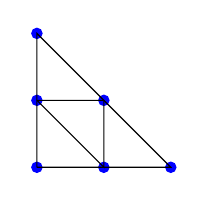
\begin{tikzpicture}[scale=1.7]

    \coordinate (0) at (0,0);
    \coordinate (1) at (1,0);
    \coordinate (2) at (0,1);

    \coordinate (3) at (0,0.5);
    \coordinate (4) at (0.5,0.5);
    \coordinate (5) at (0.5,0);

    \foreach \i in {0,1, 2, 3, 4, 5}
    \draw[blue,fill=blue] (\i) circle (1.1pt) node [below] {};


    \draw (0) --(1) -- (2) -- (0);
    \draw (3) --(4) -- (5) -- (3);

  \end{tikzpicture}
  \qquad\qquad
  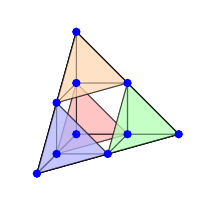
\begin{tikzpicture}[scale=1.3]

    \coordinate (0) at (0,0,0);
    \coordinate (1) at (0,0,1);
    \coordinate (2) at (1,0,0);
    \coordinate (3) at (0,1,0);
    \coordinate (4) at (0,0,0.5);
    \coordinate (6) at (0.5,0,0);
    \coordinate (7) at (0,0.5,0);
    \coordinate (5) at (0.5,0.0,0.5);
    \coordinate (8) at (0.0,0.5,0.5);
    \coordinate (9) at (0.5,0.5,0.0);

    \draw (0) -- (1) -- (2) -- (0);
    \draw (0) -- (1) -- (3) -- (0);
    \draw (1) -- (2) -- (3) -- (1);

    \draw[-, fill=red!30, opacity=.5] (4)--(6)--(7)--cycle;
    \draw[-, fill=red!30, opacity=.5] (0)--(6)--(7)--cycle;
    \draw[-, fill=red!30, opacity=.5] (0)--(4)--(7)--cycle;
    \draw[-, fill=red!30, opacity=.5] (0)--(4)--(6)--cycle;

    \draw[-, fill=blue!30, opacity=.5] (1)--(4)--(5)--cycle;
    \draw[-, fill=blue!30, opacity=.5] (1)--(4)--(8)--cycle;
    \draw[-, fill=blue!30, opacity=.5] (4)--(5)--(8)--cycle;
    \draw[-, fill=blue!30, opacity=.5] (1)--(5)--(8)--cycle;

    \draw[-, fill=green!30, opacity=.5] (2)--(5)--(6)--cycle;
    \draw[-, fill=green!30, opacity=.5] (2)--(6)--(9)--cycle;
    \draw[-, fill=green!30, opacity=.5] (2)--(5)--(9)--cycle;
    \draw[-, fill=green!30, opacity=.5] (5)--(6)--(9)--cycle;

    \draw[-, fill=orange!30, opacity=.5] (7)--(8)--(9)--cycle;
    \draw[-, fill=orange!30, opacity=.5] (3)--(7)--(9)--cycle;
    \draw[-, fill=orange!30, opacity=.5] (3)--(7)--(8)--cycle;
    \draw[-, fill=orange!30, opacity=.5] (3)--(8)--(9)--cycle;

    \foreach \i in {0,1,2,3,4,5,6,7,8,9}
    \draw[blue,fill=blue] (\i) circle (1.0pt) node [below] {};

  \end{tikzpicture}
  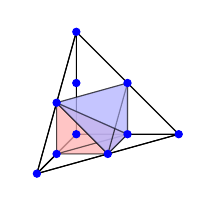
\begin{tikzpicture}[scale=1.3]

    \coordinate (0) at (0,0,0);
    \coordinate (1) at (0,0,1);
    \coordinate (2) at (1,0,0);
    \coordinate (3) at (0,1,0);
    \coordinate (4) at (0,0,0.5);
    \coordinate (6) at (0.5,0,0);
    \coordinate (7) at (0,0.5,0);
    \coordinate (5) at (0.5,0.0,0.5);
    \coordinate (8) at (0.0,0.5,0.5);
    \coordinate (9) at (0.5,0.5,0.0);

    \draw (0) -- (1) -- (2) -- (0);
    \draw (0) -- (1) -- (3) -- (0);
    \draw (1) -- (2) -- (3) -- (1);

    \draw[-, fill=red!30, opacity=.5] (4)--(5)--(6)--cycle;
    \draw[-, fill=red!30, opacity=.5] (4)--(5)--(8)--cycle;
    \draw[-, fill=red!30, opacity=.5] (4)--(6)--(8)--cycle;
    \draw[-, fill=red!30, opacity=.5] (5)--(6)--(8)--cycle;

%    \draw[-, fill=blue!30, opacity=.5] (4)--(6)--(7)--cycle;
%    \draw[-, fill=blue!30, opacity=.5] (4)--(6)--(8)--cycle;
%    \draw[-, fill=blue!30, opacity=.5] (4)--(7)--(8)--cycle;
%    \draw[-, fill=blue!30, opacity=.5] (6)--(7)--(8)--cycle;

%    \draw[-, fill=green!30, opacity=.5] (6)--(7)--(8)--cycle;
%    \draw[-, fill=green!30, opacity=.5] (6)--(7)--(9)--cycle;
%    \draw[-, fill=green!30, opacity=.5] (6)--(8)--(9)--cycle;
%    \draw[-, fill=green!30, opacity=.5] (7)--(8)--(9)--cycle;
%
    \draw[-, fill=blue!30, opacity=.5] (5)--(6)--(8)--cycle;
    \draw[-, fill=blue!30, opacity=.5] (5)--(6)--(9)--cycle;
    \draw[-, fill=blue!30, opacity=.5] (5)--(8)--(9)--cycle;
    \draw[-, fill=blue!30, opacity=.5] (6)--(8)--(9)--cycle;

    \foreach \i in {0,1,2,3,4,5,6,7,8,9}
    \draw[blue,fill=blue] (\i) circle (1.0pt) node [below] {};

  \end{tikzpicture}
  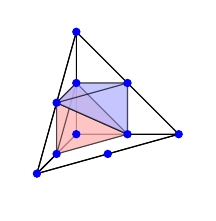
\begin{tikzpicture}[scale=1.3]

    \coordinate (0) at (0,0,0);
    \coordinate (1) at (0,0,1);
    \coordinate (2) at (1,0,0);
    \coordinate (3) at (0,1,0);
    \coordinate (4) at (0,0,0.5);
    \coordinate (6) at (0.5,0,0);
    \coordinate (7) at (0,0.5,0);
    \coordinate (5) at (0.5,0.0,0.5);
    \coordinate (8) at (0.0,0.5,0.5);
    \coordinate (9) at (0.5,0.5,0.0);

    \draw (0) -- (1) -- (2) -- (0);
    \draw (0) -- (1) -- (3) -- (0);
    \draw (1) -- (2) -- (3) -- (1);

%    \draw[-, fill=red!30, opacity=.5] (4)--(5)--(6)--cycle;
%    \draw[-, fill=red!30, opacity=.5] (4)--(5)--(8)--cycle;
%    \draw[-, fill=red!30, opacity=.5] (4)--(6)--(8)--cycle;
%    \draw[-, fill=red!30, opacity=.5] (5)--(6)--(8)--cycle;

    \draw[-, fill=red!30, opacity=.5] (4)--(6)--(7)--cycle;
    \draw[-, fill=red!30, opacity=.5] (4)--(6)--(8)--cycle;
    \draw[-, fill=red!30, opacity=.5] (4)--(7)--(8)--cycle;
    \draw[-, fill=red!30, opacity=.5] (6)--(7)--(8)--cycle;

    \draw[-, fill=blue!30, opacity=.5] (6)--(7)--(8)--cycle;
    \draw[-, fill=blue!30, opacity=.5] (6)--(7)--(9)--cycle;
    \draw[-, fill=blue!30, opacity=.5] (6)--(8)--(9)--cycle;
    \draw[-, fill=blue!30, opacity=.5] (7)--(8)--(9)--cycle;

%    \draw[-, fill=orange!30, opacity=.5] (5)--(6)--(8)--cycle;
%    \draw[-, fill=orange!30, opacity=.5] (5)--(6)--(9)--cycle;
%    \draw[-, fill=orange!30, opacity=.5] (5)--(8)--(9)--cycle;
%    \draw[-, fill=orange!30, opacity=.5] (6)--(8)--(9)--cycle;

    \foreach \i in {0,1,2,3,4,5,6,7,8,9}
    \draw[blue,fill=blue] (\i) circle (1.0pt) node [below] {};

  \end{tikzpicture}

  \caption{New refinement strategies for triangles and tetrahedrons: triangles
  are subdivided in 4 children and tetrahedrons in 8 ones.}\label{fig:refinement}

\end{figure}

\begin{itemize}
\item Experimental support of locally refined meshes. FEM on locally refined
meshes requires 1) the possibility to locally refine the mesh (see Figure~\ref{fig:refinement})
and 2) appropriate hanging-node constraints. For 3D, the implementation of the missing constraint definitions is in progress.
\item TODO
\end{itemize}

Furthermore, we continued to remove the instance of usage of the \texttt{GeometryInfo} class from
the library and to replace them by more general equivalent functions, which
rely on \texttt{ReferenceCell} in many cases. Once all instances of
\texttt{GeometryInfo} are removed, we will deprecate the class.

%%%%%%%%%%%%%%%%%%%%%%%%%%%%%%%%%%%%%%%%%%%%%%%%%%%%%%%%%%%%%%%%%%%%%%%%%%%%%%%%
\subsection{Repartitioning of distributed meshes}\label{sec:repartitioning}

Until now, distributed meshes were either partitioned statically (\texttt{parallel::\allowbreak fullydistributed::\allowbreak Triangulation}; short \texttt{p::f::T}) or they used a
fixed policy to partition the cells among processes
(\texttt{parallel::\allowbreak distributed::\allowbreak Triangulation}; short \texttt{p::d::T}). For the latter, we
use the Morton-order as the backend \texttt{p4est} does. A fixed Morton-order
might provide very good performance in terms in communication and
setup costs, but might be non-optimal when interfacing with other
libraries that have fixed partitioning, e.g., a Cartesian
partitioning, themselves.

New utility functions from the \texttt{RepartitioningPolicyTools} namepace can be
used now to create a new \texttt{p::f::T} instance,
given a distributed triangulation (\texttt{p::f::T} or \texttt{p::d::T}) and a vector with the new owners of locally
owned cells. The workflow is shown in the following listing:
\begin{c++}
// original triangulation
parallel::distributed::Triangulation<dim> tria(comm);

// select a partitioning policy and use it
const RepartitioningPolicyTools::Cartesian<dim> policy(tria);
const auto construction_data = TriangulationDescription::Utilities::
  create_description_from_triangulation(tria, policy.partition(tria));

// create the new triangulation
parallel::fullydistributed::Triangulation<dim> tria_pft(comm);
tria_pft.create_triangulation(construction_data);
\end{c++}
Instead of using one of the predefined partitioning policies, users
can write their own ones by implementing the \texttt{RepartitioningPolicyTools::Base} interface. Similarly to the
active level, also the multigrid levels can be repartitioned arbitrarily.

\begin{figure}
    \centering
    \def\svgwidth{0.8\columnwidth}
    \input{svg/repartitioning.pdf_tex}
    \caption{Visualization of the repartitioning process: after new ranks
    are assigned to cells, each process collects and sends the cells, incl.
    ghost cells, to the new owner. There, incoming cells are processed, duplicates
    are removed, and the local part of the triangulation is built.}\label{fig:repartitioning}
\end{figure}

The setup process is visualized in Figure~\ref{fig:repartitioning}. At first, cells, including their
surrounding (ghost) cells and parent cells, are collected and
sent to the new owner. On the
receiving site, the sets of all cells are combined and possible duplicates
are removed. This information is enough to construct a new triangulation.
For sending/receiving, we apply consensus-based algorithms~\cite{hoefler2010scalable}, which
we introduced into the library in release 9.2~\cite{dealII92} -- see
also Section~\ref{sec:CA}. Consensus-based
algorithms are used also in \cite{ibanez2016pumi} for repartitioning.

In future releases, we plan to add support for repartitioning based on distributed graph
partitioning libraries, e.g., \texttt{ParMETIS} or \texttt{Zoltan}. Furthermore, we intend to extend
\texttt{p::f::T} with adaptivity support.
With this support and and the new repartitioning features, \texttt{p::f::T}
could be self-consistent like \texttt{p::d::T}, which is an important
step towards the support of AMR also for distributed simplex and mixed meshes
(see also Subsection~\ref{sec:simplex}).

%We would like to note that we provide a similar class also for repartitioning
%of vectors: \texttt{Noncontiguous\allowbreak Partitioner} from the
%\texttt{Utilities::MPI} namespace.

%%%%%%%%%%%%%%%%%%%%%%%%%%%%%%%%%%%%%%%%%%%%%%%%%%%%%%%%%%%%%%%%%%%%%%%%%%%%%%%%
\subsection{Advances in matrix-free infrastructure}\label{sec:mf}

In the matrix-free infrastructure, we have added a number of new features. The most
notable ones are:
\begin{itemize}
\item Improved support of computations with Hessians of shape functions: just like values and gradients, Hessians can be
now evaluated and integrated during matrix-free loops
both for cells and faces. This enables, e.g., to write
a matrix-free version of step-47, which solves the biharmonic equation with DG.
\item Cell-centric loops now also allow to access gradients and Hessians
of neighboring cells on faces. The major difficulty here was their reorientation
in the case of arbitrary orientated cells on unstructured meshes.
\item Users can now create their own cell batches, by providing \texttt{FEEvaluation::reinit()} a list of cell IDs. \texttt{FEEvaluation}
accesses the appropriate data and reshuffles mapping data accordingly on
the fly in order to enable vectorization over cells. The new feature is useful in many
contexts. Examples are application with sharp interfaces (e.g., two-phase flow
or shock capturing), where one needs to treat cells that are ``cut'' by
the interface in a special way. A challenge is that cell batches
might contain cut or not-cut cells, making vectorization potentially more complicated. One way to deal with such cell batches is to apply masks if
the code paths do not diverge too much
(a lot of functions of \texttt{FEEvaluation} allows this). Another way is to
categorize cells during \texttt{MatrixFree::reinit()} in such a way that mixed cell batches do not occur. However, calling  \texttt{MatrixFree::reinit()}
might be too expensive if a very dynamic system is given, which requires
recategorization in each time step. Doing this on the fly might be a cheep alternative, even if not computationally optimal during matrix-free loops.
\item Initial support for H(div)-conforming elements with Piola transform, based on Raviart--Thomas finite element spaces with the updated class \texttt{FE\_RaviartThomasNodal}, has been added. The features are currently limited to meshes in standard orientations and affine geometries. Full support will be provided in the next release.
\item Selected matrix-free algorithms can now exploit additional data locality
  between the matrix-vector product and vector operations happening nearby in
  an algorithms. These have been added to both the
  \texttt{PreconditionChebyshev} class often used as a smoother in multigrid
  methods and the conjugate gradient implementation in \texttt{SolverCG}. To
  use these features, an operator needs to define a \texttt{vmult} operation,
  taking two additional \texttt{std::function} arguments. The first function
  defines what should be scheduled on the vector entries before the
  matrix-vector product touches them, and the second what happens
  afterwards. The new features also include a renumbering to maximize data
  locality. The theory is described in the
  contribution~\cite{kronbichler2022cg}.
\todo[inline]{We could also make this last a separate section or in the introduction, but it feels it fits well here.}
\end{itemize}
Besides these new features, we improved the performance of
hanging-node-constraint evaluation on the CPU. Instead of performing
quasi-dense matrix-vector multiplications~\cite{KronbichlerKormann2012}, we now use an
approach based on inplace interpolation and sumfactorization, similarly
as we already did in the GPU code~\cite{ljungkvist2017matrix}. In \cite{munch2022hn}, the algorithm is described
and performance numbers are shown, indicating a reduction
of overhead of cells with hanging nodes by a factor of 10$\times$.

Furthermore, we have performed a major restructuring of internals
of the \texttt{FEEvaluation} classes. This will enable us to add the support of new element types, e.g., of
Raviart--Thomas and Nedelec elements,  more
simply in the future.


%\begin{c++}
%additional_data.mapping_update_flags = ... | update_hessians;
%\end{c++}
%
%\begin{c++}
%FEEvaluation<dim> phi(matrix_free);
%
%phi.reinit(cell);
%phi.gather_evaluate(src, ... | EvaluationFlags::hessians);
%
%for(const auto q : phi.quadrature_point_indices())
%  phi.submit_hessian(phi.get_hessian(q), q);
%
%phi.integrate_scatter(... | EvaluationFlags::hessians, dst);
%\end{c++}
%
%... similar for faces; can be used to implement biharmonic equation (like in
%step-X)


%%%%%%%%%%%%%%%%%%%%%%%%%%%%%%%%%%%%%%%%%%%%%%%%%%%%%%%%%%%%%%%%%%%%%%%%%%%%%%%%
\subsection{Advances in multigrid infrastructure}\label{sec:multigrid}

In release 9.3~\cite{dealII93}, we added support for global-coarsening multigrid in
addition to the established local-smoothing infrastructure. Global
coarsening smoothens on the whole computational domain on each
multigrid level, which is obtained by coarsening the finest mesh globally.
For this purpose, we use a sequence of triangulations, and we perform
the smoothing only on their active levels. To create the sequence of
triangulations, one can use the functions \texttt{create\_geometric\_coarsening\_sequence()} from the
\texttt{MGTransferGlobalCoarseningTools} namespace. A new version takes an
instance of \texttt{RepartitioningPolicyTools::Base} (see Subsection~\ref{sec:repartitioning}) as argument, which allows to specify the parallel
distribution of each multigrid level (in contrast to the fixed first-child policy in the case of local smoothing). Furthermore, we added support for block vectors,
fixed a number of limitations, and performed performance optimizations of
the transfer operator; particularly, the redundant copy from/to temporary vectors
has been eliminated. Now, hanging-node constraints are applied
efficiently in the same way as in the matrix-free loops (see Subsection~\ref{sec:mf}).

In \cite{munch2022gc}, the performance of the local-smoothing and global-coarsening
infrastructure of \texttt{deal.II} was compared for locally refined meshes. The results indicate that
the local definition of multigrid levels might introduce load imbalances
in the case of local smoothing so that global coarsening is favorable despite
potentially more expensive intergrid transfers. In order to judge the benefits
of one approach against the other, \texttt{deal.II} provides new functions
\texttt{workload\_imbalance()} and \texttt{vertical\_communication\_efficiency()}
in the \texttt{MGTools} namespace for the  estimation of the workload imbalance and the
vertical communication efficiency purely based on the given mesh. The publication \cite{munch2022gc} also points out that not
all types of smoothers are applicable for global coarsening due to the
presence of hanging nodes, which is a motivation to add new smoother types
to \dealii in the future.

%%%%%%%%%%%%%%%%%%%%%%%%%%%%%%%%%%%%%%%%%%%%%%%%%%%%%%%%%%%%%%%%%%%%%%%%%%%%%%%%
\subsection{CutFEM support}\label{sec:cut}

Several classes have been added to the \texttt{NonMatching} namespace to enable the use of cut finite element methods~\cite{burman_cutfem_2015}.
In the literature, these types of methods are also referred to as immersed, extended, or fictitious finite element methods.
Here, the domain, $\Omega$, is immersed in the background mesh, as illustrated in Figure~\ref{fig:immersed-domain}.
Often, one solves for the degrees of freedom of the smallest submesh which completely covers the domain.
The bilinear form in the weak form can, for example, look like
\begin{equation}
  a(u,v) = (\nabla u, \nabla v)_\Omega - (\partial_n u, v)_\Gamma + \ldots
\end{equation}
Thus, when assembling, we are on each cell
required to integrate over the part of the domain and the part of the boundary, $\Gamma = \partial \Omega$, that falls inside the cell:
$K\cap \Omega$ and $K \cap \Gamma$.
Many of the new classes assume that the domain is described by a level set function,
$\psi : \mathbb{R}^d \to \mathbb{R}$, such that
\begin{align}
  \Omega = \{x \in \mathbb{R}^d : \psi(x)<0\},
  \qquad
  \Gamma = \{x \in \mathbb{R}^d : \psi(x) = 0\}.
\end{align}
\begin{itemize}
  \item The \texttt{MeshClassifier} class identifies how the active cells and faces are located relative to the zero contour of the level set function, as illustrated in Figure~\ref{fig:location-to-level-set}. Its \texttt{location\_to\_level\_set} function takes a cell/face and
        returns an enum, \texttt{LocationToLevelSet}, which takes values \{\texttt{inside}, \texttt{outside}, \texttt{intersected}\}.
        These indicate whether $\psi$ is negative, positive, or varies in sign over the cell/face.
        That is, the cell/face is located inside/outside $\Omega$, or is intersected by $\Gamma$.
        This information is typically needed when choosing what element a cell of the \texttt{DoFHandler} should use.

  \item The \texttt{QuadratureGenerator} class, which implements the algorithm in \cite{saye2015}, generates high-order quadrature rules for the 3 different regions of a \texttt{BoundingBox}, $B$, defined by the sign of the level set function:
        \begin{align}
          B \cap \Omega = \{ x\in B:  \psi(x) < 0 \},  \quad
          B \cap \Gamma = \{ x\in B:  \psi(x) = 0 \},  \quad
          \{ x\in B:  \psi(x) > 0 \}.
        \end{align}
        An example of these quadratures is shown in Figure~\ref{fig:immersed_quadratures}.
        Correspondingly, the \newline \texttt{FaceQuadratureGenerator} class generates the same type of quadratures but over a face of $B$.
        Furthermore, the new classes \texttt{DiscreteQuadratureGenerator} and \newline \texttt{DiscreteFaceQuadratureGenerator} can be used to generate these quadrature rules over a cell/face when the level set function lies in a finite element space: $\psi_h \in V_h$, and when the reference cell of the cell/face is a hypercube.

  \item \texttt{ImmersedSurfaceQuadrature} is a class representing a quadrature rule over a $(d-1)$-dimensional surface embedded in $\mathbb{R}^d$ ($\psi = 0$ in Figure~\ref{fig:immersed_quadratures}). In addition to the weight, it stores the unit normal to the surface, for each quadrature point. This is needed to be able to transform the quadrature rule from reference space to real space.

  \item \texttt{FEImmersedSurfaceValues} is a \texttt{FEValues}-like class for evaluating real space values based on an \texttt{ImmersedSurfaceQuadrature}.

  \item \texttt{NonMatching::FEValues} combines the functionality of several of the above classes to simplify assembling. It works similarly to \texttt{hp::FEValues}.
  When calling the \texttt{reinit} function, the immersed quadrature rules are generated in the background and
  \texttt{dealii::FEValues} objects for the inside/outside region and a \texttt{FEImmersedSurfaceValues} object for the surface regions are set up internally. These can then be obtained using getter-functions and used for the assembly.
  Since the generation of immersed quadrature rules is not for free,
  \texttt{NonMatching::FEValues} calls  \texttt{QuadratureGenerator} only if it is needed, i.e. if the cell is intersected. If the cell passed to \texttt{reinit} is not intersected, already cached \texttt{dealii::FEValues} objects will be returned by the getter functions.
  Correspondingly, the class \texttt{NonMatching::FEInterfaceValues} generates
  \texttt{dealii::FEInterfaceValues} objects for assembling face terms of the type $F \cap \{x : \psi(x) < 0 \}$ or $F \cap \{x : \psi(x) > 0 \}$.
\end{itemize}
The new \texttt{step-85} tutorial shows how many of these classes go together.

\begin{figure}[h]
  \centering
  \begin{subfigure}[b]{0.3\textwidth}
    \centering
    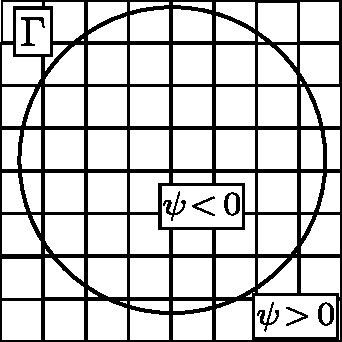
\includegraphics[height=.12\paperheight]{svg/immersed-domain.pdf}
    \caption{\label{fig:immersed-domain}}
  \end{subfigure}
  \qquad
  \begin{subfigure}[b]{0.3\textwidth}
    \centering
    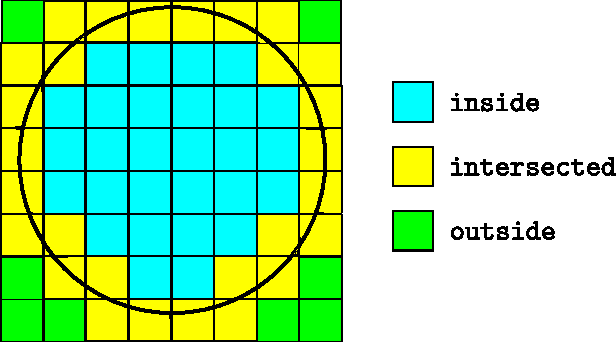
\includegraphics[height=.12\paperheight]{svg/location-to-level-set.pdf}
    \caption{ \label{fig:location-to-level-set}}
  \end{subfigure}
  \caption{a) Domain immersed in a background mesh. b) Value of \texttt{LocationToLevelSet} for each cell}
\end{figure}

\begin{figure}[h]
  \centering
  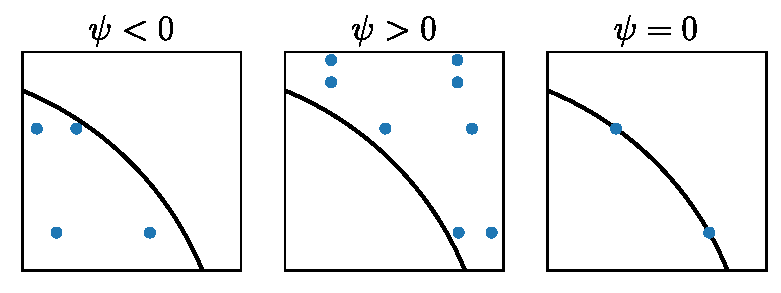
\includegraphics[width=.4\paperwidth]{svg/immersed_quadratures.pdf}
  \caption{Quadrature points for integrating over the three different regions of a cell cut by the zero contour of the level set function, $\psi$. \label{fig:immersed_quadratures}}
\end{figure}



%%%%%%%%%%%%%%%%%%%%%%%%%%%%%%%%%%%%%%%%%%%%%%%%%%%%%%%%%%%%%%%%%%%%%%%%%%%%%%%%
\subsection{Integration with the Computational Geometry Algorithms
  Library (CGAL)}\label{sec:cgal}

\begin{itemize}
\item new classes
\end{itemize}

%%%%%%%%%%%%%%%%%%%%%%%%%%%%%%%%%%%%%%%%%%%%%%%%%%%%%%%%%%%%%%%%%%%%%%%%%%%%%%%%
\subsection{Performance improvement of particle infrastructure}\label{sec:particles}

\begin{itemize}
\item describe the new data structure
\item do we have performance numbers?
\end{itemize}



%%%%%%%%%%%%%%%%%%%%%%%%%%%%%%%%%%%%%%%%%%%%%%%%%%%%%%%%%%%%%%%%%%%%%%%%%%%%%%%%
\subsection{Improvements to unstructured communication}
\label{sec:CA}

\todo[inline]{Wolfgang to write something about the CA algorithms (and to give
credit to the previous implementation by Peter). Mention improvements
to pack(), unpack(), broadcast() too.}

Also reference Section~\ref{sec:repartitioning}.


%%%%%%%%%%%%%%%%%%%%%%%%%%%%%%%%%%%%%%%%%%%%%%%%%%%%%%%%%%%%%%%%%%%%%%%%%%%%%%%%
\subsection{Topic 7}



%%%%%%%%%%%%%%%%%%%%%%%%%%%%%%%%%%%%%%%%%%%%%%%%%%%%%%%%%%%%%%%%%%%%%%%%%%%%%%%%
\subsection{New and improved tutorials and code gallery programs}
\label{subsec:steps}

Many of the \dealii{} tutorial programs were revised in a variety of
ways as part of this release. In addition, there are a number of new tutorial programs:
\begin{itemize}
\item \texttt{step-82} was contributed by Andrea Bonito (Texas A\&M University) and Diane Guignard (University of Ottawa). It shows how
\dealii{} can be used to implement the
local discontinuous Galerkin (LDG) method for approximating the solution to the bi-Laplacian problem.
\item \texttt{step-85} was contributed by Simon Sticko (Uppsala University). It shows how to use the new CutFEM infrastructure to solve a Poisson
problem on a circular domain that is embedded in a Cartesian background mesh.
\end{itemize}

There is also a new program in the code gallery (a collection of
user-contributed programs that often solve more complicated problems
than tutorial programs, and intended as starting points for further
research rather than as teaching tools):
\begin{itemize}
\item ``\texttt{MCMC for the Laplace equation}'' TODO.
\end{itemize}



%%%%%%%%%%%%%%%%%%%%%%%%%%%%%%%%%%%%%%%%%%%%%%%%%%%%%%%%%%%%%%%%%%%%%%%%%%%%%%%%
\subsection{Incompatible changes}\label{subsec:deprecated}

The 9.4 release includes
\href{https://dealii.org/developer/doxygen/deal.II/changes_between_9_3_0_and_9_4_0.html}
{around 40 incompatible changes}; see \cite{changes94}. The majority of these changes
should not be visible to typical user codes; some remove previously
deprecated classes and functions; and the majority changes internal
interfaces that are not usually used in external
applications. That said, the following are worth mentioning since they
may have been more widely used:
\begin{itemize}
  \item In continuation of our attempt to merge the classes \texttt{DoFHandler} and \texttt{hp::DoFHandler}, we have removed the
  template parameter \texttt{DoFHandlerType} from number of classes and
  functions and replaced it by \texttt{dim}/\texttt{spacedim}. Affected
  classes are, e.g., \texttt{SolutionTransfer} and \texttt{DataOut}.
  \item \texttt{FE\_RaviartThomasNodal} now uses a different polynomial space to allow
  for a simpler use for faces in non-standard orientation. The new polynomials
  are anisotropic tensor products of Lagrange polynomials on the points of the
  Gauss--Lobatto quadrature formula. This change leads to different entries, for example, in
  the matrices and constraints, but no change in accuracy should be expected as the resulting polynomial
  space spans the same polynomials.
  \item The class \texttt{MappingQ} now applies a high-order mapping to all cells, not just the cells near the boundary, functionality that was previously provided by the \texttt{MappingQGeneric} class. The latter has been marked as deprecated. In order to use different degrees for the mapping, users can use \texttt{hp::MappingCollection} or \texttt{MappingFEField} with appropriate definitions of function spaces.
  \item We made different changes in the repartitioning of \texttt{parallel::distributed::Triangulation}.
  Most notably, we have removed the default weight in order to ensure consistency with the rest of the
  library.
\end{itemize}



%%%%%%%%%%%%%%%%%%%%%%%%%%%%%%%%%%%%%%%%%%%%%%%%%%%%%%%%%%%%%%%%%%%%%%%%%%%%%%%%
%%%%%%%%%%%%%%%%%%%%%%%%%%%%%%%%%%%%%%%%%%%%%%%%%%%%%%%%%%%%%%%%%%%%%%%%%%%%%%%%
%%%%%%%%%%%%%%%%%%%%%%%%%%%%%%%%%%%%%%%%%%%%%%%%%%%%%%%%%%%%%%%%%%%%%%%%%%%%%%%%
\section{How to cite \dealii}\label{sec:cite}

In order to justify the work the developers of \dealii{} put into this
software, we ask that papers using the library reference one of the
\dealii{} papers. This helps us justify the effort we put into this library.

There are various ways to reference \dealii{}. To acknowledge the use of
the current version of the library, \textbf{please reference the present
  document}. For up to date information and a bibtex entry
see
\begin{center}
  \url{https://www.dealii.org/publications.html}
\end{center}

The original \dealii{} paper containing an overview of its
architecture is \cite{BangerthHartmannKanschat2007}, and a more recent
publication documenting \dealii{}'s design decisions is available as \cite{dealII2020design}. If you rely on
specific features of the library, please consider citing any of the
following:
\begin{multicols}{2}
  \vspace*{-36pt}
  \begin{itemize}
    \item For geometric multigrid: \cite{Kanschat2004,JanssenKanschat2011,ClevengerHeisterKanschatKronbichler2019, munch2022gc};
    \item For distributed parallel computing: \cite{BangerthBursteddeHeisterKronbichler11};
    \item For $hp$-adaptivity: \cite{BangerthKayserHerold2007};
    \item For partition-of-unity (PUM) and finite element enrichment methods:
           \cite{Davydov2016};
    \item For matrix-free and fast assembly techniques:
          \cite{KronbichlerKormann2012,KronbichlerKormann2019};
    \item For computations on lower-dimensional manifolds:
          \cite{DeSimoneHeltaiManigrasso2009};
    \item For curved geometry representations and manifolds:
          \cite{HeltaiBangerthKronbichlerMola2019};
    \item For integration with CAD files and tools:
          \cite{HeltaiMola2015};
    \item For boundary element computations:
          \cite{GiulianiMolaHeltai-2018-a};
    \item For the \texttt{LinearOperator} and
      \texttt{Packaged\-Operation} facilities:
          \cite{MaierBardelloniHeltai-2016-a,MaierBardelloniHeltai-2016-b};
    \item For uses of the \texttt{WorkStream} interface:
          \cite{TKB16};
    \item For uses of the \texttt{ParameterAcceptor} concept, the
          \texttt{MeshWorker::ScratchData} base class, and the
          \texttt{ParsedConvergenceTable} class:
          \cite{SartoriGiulianiBardelloni-2018-a};
    \item For uses of the particle functionality in \dealii{}:
          \cite{GLHPB18}.
          \vfill\null
  \end{itemize}
\end{multicols}

\dealii{} can interface with many other libraries:
\todo[inline]{Need to update, in particular add CGAL.}
\begin{multicols}{3}
  \begin{itemize}
    \item ADOL-C \cite{Griewank1996a,adol-c}
    \item ArborX \cite{lebrun2020arborx}
    \item ARPACK \cite{arpack}
    \item Assimp \cite{assimp}
    \item BLAS and LAPACK \cite{lapack}
    \item cuSOLVER \cite{cusolver}
    \item cuSPARSE \cite{cusparse}
    \item Gmsh \cite{geuzaine2009gmsh}
    \item GSL \cite{gsl2016}
    \item Ginkgo \cite{ginkgo-web-page}
    \item HDF5 \cite{hdf5}
    \item METIS \cite{karypis1998fast}
    \item MUMPS \cite{ADE00,MUMPS:1,MUMPS:2,mumps-web-page}
    \item muparser \cite{muparser-web-page}
    \item OpenCASCADE \cite{opencascade-web-page}
    \item p4est \cite{p4est}
    \item PETSc \cite{petsc-user-ref,petsc-web-page}
    \item ROL \cite{ridzal2014rapid}
    \item ScaLAPACK \cite{slug}
    \item SLEPc \cite{Hernandez:2005:SSF}
    \item SUNDIALS \cite{sundials}
    \item SymEngine \cite{symengine-web-page}
    \item TBB \cite{Rei07}
    \item Trilinos \cite{trilinos,trilinos-web-page}
    \item UMFPACK \cite{umfpack}
  \end{itemize}
\end{multicols}
Please consider citing the appropriate references if you use
interfaces to these libraries.

The two previous releases of \dealii{} can be cited as
\cite{dealII92,dealII93}.


\section{Acknowledgments}

\dealii{} is a world-wide project with dozens of contributors around the
globe. Other than the authors of this paper, the following people
contributed code to this release:\\
%
% Uwe Koecher doesn't usually show up in the changelog, but
% we should make sure he's listed.
%
\todo[inline]{updated 23/04/2022 PM. We should probably make sure that
  nobody else came after that and before the release.}
Pasquale	Africa,
Tyler	Anderson,
Francesco	Andreuzzi,
Mathias	Anselmann,
Maximilian	Bergbauer,
Bruno	Blais,
Till	Budde,
Fabian	Castelli,
Praveen	Chandrashekar,
Cu	Cui,
Ivo	Dravins,
Niklas	Fehn,
Johannes	Friedlein,
Sebastian	Fuchs,
Rene	Gassmoeller,
Nicola	Giuliani,
Alexander	Grayver,
Diane	Guignard,
Jake	Harmon,
Sean	Ingimarson,
Pengfei	Jia,
Sebastian	Kinnewig,
Simon	Konrad,
Katharina	Kormann,
Paras	Kumar,
Wenyu	Lei,
Alberto F.	Martin,
Nils	Much,
Lucas	Myers,
Justin	O'Connor,
Judith	Pauen,
Vachan	Potluri,
Raghunandan	Pratoori,
Sebastian	Proell,
Ce	Qin,
Reza	Rastak,
Jose E.	Roman,
Raphael	Schoof,
Magdalena	Schreter,
Konrad	Simon,
Simon	Sticko,
Bruno	Turcksin,
Kuljit S.	Virk,
Michał	Wichrowski,
Niklas Wik,
Jiaqi	Zhang.


Their contributions are much appreciated!


\bigskip

\dealii{} and its developers are financially supported through a
variety of funding sources:

\todo[inline]{Update. In particular make sure that we remove those who
  are not authors on this paper.}

D.~Arndt and B.~Turcksin: Research sponsored by the Laboratory Directed Research and
Development Program of Oak Ridge National Laboratory, managed by UT-Battelle,
LLC, for the U. S. Department of Energy.

W.~Bangerth, T.~Heister, R.~Gassm{\"o}ller, and J.~Zhang were partially
supported by the Computational Infrastructure for Geodynamics initiative
(CIG), through the National Science Foundation (NSF) under Award
No.~EAR-1550901 and The University of California -- Davis.

W.~Bangerth and M.~Fehling were partially supported by Award OAC-1835673
as part of the Cyberinfrastructure for Sustained Scientific Innovation (CSSI)
program.

W.~Bangerth was also partially supported by Awards DMS-1821210 and EAR-1925595.

B.~Blais was partially supported by the National Science and Engineering
Research Council of Canada (NSERC)  through the RGPIN-2020-04510 Discovery
Grant

T.~Heister and J.~Zhang were also partially supported by NSF
Award OAC-2015848.

T.~Heister was also partially supported by the NSF Awards DMS-2028346,
EAR-1925575, and by Technical Data Analysis, Inc. through US Navy STTR
Contract N68335-18-C-0011.

R.~Gassm{\"o}ller was also partially supported by the NSF Award
EAR-1925595.

L.~Heltai was partially supported by the Italian Ministry of Instruction,
University and Research (MIUR), under the 2017 PRIN project NA-FROM-PDEs MIUR
PE1, ``Numerical Analysis for Full and Reduced Order Methods for the efficient
and accurate solution of complex systems governed by Partial Differential
Equations''.

M.~Kronbichler and P.~Munch were partially supported by the
Bayerisches Kompetenznetzwerk
f\"ur Technisch-Wissen\-schaft\-li\-ches Hoch- und H\"ochstleistungsrechnen
(KONWIHR) in the context of the projects
``High-order matrix-free finite element implementations with
hybrid parallelization and improved data locality'' and ``Fast and scalable finite element algorithms for coupled multiphysics problems and non-matching grids''.

M.~Maier was partially supported by NSF Awards DMS-1912847 and DMS-2045636.

S.~Sticko was partially supported by eSSENCE of e-Science.

D.~Wells was supported by NSF through Grant DMS-1344962.

The Interdisciplinary Center for Scientific Computing (IWR) at Heidelberg
University has provided hosting services for the \dealii{} web page.

\bibliography{paper}{}
\bibliographystyle{abbrv}

\end{document}
